\section{Introduction and results}

The edge version of inducibility asks how many induced copies of a fixed
graph can occur in a graph with a prescribed number of edges. Recent work
of Wang, Zhao, and Lu~\cite{Wang2026} and of Chao, Cohen Antonir, Li, and
Yu~\cite{Chao2025} studies this problem through entropy inequalities and
local directed graphs. For the pentagon, both works conjecture that balanced
blow-ups of \(C_5\) give the asymptotically optimal count
\((m/5)^{5/2}\); see \cite[Conjecture~8]{Wang2026} and
\cite[Conjecture~1.7]{Chao2025}. We determine the sharp constant, which is
larger by a factor of \(3/(2\sqrt{2})\), and prove the corresponding rigidity
and stability statements. We then resolve the second-order arithmetic
oscillation and obtain an eventual exact polynomial at each fixed offset
from the equality sequence.

The extremal construction itself is known. Davey, Hurley, de Joannis de
Verclos, Kang, and Volec~\cite[Lemmas~1.4, 7.1, and 7.2]{Davey2026} record
the Clebsch pentagon count and its balanced blow-ups while studying
triangle-free pentagon counts normalized by \(|G|\Delta(G)^4\). Our upper
bound concerns arbitrary graphs with a prescribed edge count. We include
the elementary construction count below to fix the normalization.

With the number of vertices prescribed, the induced-pentagon problem has
a different extremal structure. Balogh, Hu, Lidick\'y, and
Pfender~\cite{Balogh2016} established the asymptotic result using iterated
\(C_5\) blow-ups; Lidick\'y, Mattes, and Pfender~\cite{Lidicky2023}
subsequently determined the extremal count for every order. Those results
provide context for the induced-count problem. Here the active vertex count
is part of the optimization and may be accompanied by an arbitrary number
of isolated vertices.

Let \(H\) be a finite simple graph with nonnegative vertex weights
\(x=(x_v)_{v\in V(H)}\). Define
\[
 E(H,x)=\sum_{uv\in E(H)}x_ux_v,\qquad
 C(H,x)=\sum_{\substack{U\subseteq V(H)\\ H[U]\cong C_5}}
                  \prod_{v\in U}x_v .
\]
Thus all pentagons counted by \(C\) are induced, including when \(H\)
contains triangles. Set
\[
 c_*=\frac{3}{50\sqrt{10}}=\frac{192}{40^{5/2}},
 \qquad
 R_*=\frac{3}{2\sqrt{2}}=5^{5/2}c_*.
\]
The Clebsch graph is the Cayley graph on \(\mathbb F_2^4\) generated by
\[
 \{e_1,e_2,e_3,e_4,e_1+e_2+e_3+e_4\}.
\]
It has degree five and forty edges. The only nonempty linear dependence
among these five generators is their full sum. Every closed walk of length
five therefore uses all five generators once and is a simple pentagon.
There are \(16\cdot 5!/10=192\) pentagons, and there are no triangles.
Every pentagon is induced.

\begin{theorem}[Sharp weighted bound and equality]\label{thm:weighted}
Every finite simple graph with nonnegative vertex weights satisfies
\begin{equation}
 C(H,x)\le c_*E(H,x)^{5/2}.\tag{1}\label{eq:weighted}
\end{equation}
If \(E(H,x)>0\), equality holds if and only if, after zero-weight vertices
are discarded, the graph consists of a Clebsch blow-up and isolated vertices,
with the sixteen Clebsch classes having equal total weight.
\end{theorem}

Write \(I_5(G)\) for the number of induced pentagons in an ordinary graph.
A graph with \(m>0\) edges satisfies
\[
 I_5(G)\le R_*\left(\frac m5\right)^{5/2}.
\]
Equality holds exactly for a Clebsch blow-up with the same positive integer
number \(k\) of vertices in every class, together with isolates. Such a
graph has \(40k^2\) edges and \(192k^5\) induced pentagons.

\begin{corollary}[Asymptotic edge inducibility]\label{cor:asymptotic}
If \(\rho(C_5,m)\) is the largest number of induced pentagons in a graph
with exactly \(m\) edges, then
\[
 \rho(C_5,m)=c_*m^{5/2}+O(m^2).
\]
\end{corollary}
\begin{proof}
The upper bound is Theorem~1.1. For the lower bound, take a balanced
Clebsch blow-up with \(k=\lfloor\sqrt{m/40}\rfloor\) and add a disjoint
matching with \(m-40k^2\) edges. It has exactly \(m\) edges and \(192k^5\)
induced pentagons. Since \(m-40k^2=O(\sqrt m)\), the asserted error follows.
\end{proof}

In the normalization of~\cite{Chao2025}, our result reads
\[
 \operatorname{eind}(C_5)
 =\limsup_{m\to\infty}\frac{10\rho(C_5,m)}{(2m)^{5/2}}
 =\frac{3}{40\sqrt5}.
\]
The upper bound in \cite[Theorem~1.8]{Chao2025} is \(1/\sqrt{250}\) in this
normalization. Thus the sharp bound also settles the pentagon case
identified as open in that paper.

For a graphon \(W:[0,1]^2\to[0,1]\), use the normalization
\[
 \begin{gathered}
 E(W)=\frac12t(K_2,W),\qquad
 C(W)=\frac1{10}t_{\mathrm{ind}}(C_5,W),\\
 R(W)=5^{5/2}\frac{C(W)}{E(W)^{5/2}}.
 \end{gathered}
\]
Let \(\mathcal E_{\mathrm{Cl}}\) be the family obtained by partitioning an
active set of arbitrary positive measure into sixteen equal classes,
placing Clebsch adjacency between them, and making all remaining points
isolated.

\begin{theorem}[Graphon bound and equality]\label{thm:graphon}
Every positive-density graphon satisfies \(R(W)\le R_*\).
Equality holds exactly for \(\mathcal E_{\mathrm{Cl}}\), up to a measurable
partition and null sets. In particular every equality graphon is
\(\{0,1\}\)-valued.
\end{theorem}

The stability statement is on the edge scale. If
\(I_5(G)\ge (R_*-\varepsilon)(m/5)^{5/2}\), then
\(O(\sqrt{\varepsilon}\,m)\) edge additions and deletions suffice to obtain
an exactly balanced Clebsch blow-up and isolates on the original vertex
set. Theorem~8.1 states this precisely. There is no bound on the original
number of vertices and no additional rounding error. The exponent \(1/2\)
cannot be improved.

Our stronger structural conclusion distinguishes adjacency errors from
class imbalance. A graph with normalized deficit \(\varepsilon\) can be
edited into a possibly unbalanced Clebsch blow-up with integer class sizes
\(n_i\), total active size \(N\), and
\[
 |E(G)\mathbin{\triangle}E(H)|
       +\sum_{i=1}^{16}(n_i-N/16)^2=O(\varepsilon m).
\]
There is no additive rounding loss. We also prove a two-sided comparison
between the pentagon deficit and this structural quantity; see Section~9.

The integer edge count produces a nonconstant second-order term. Writing
\[
 \alpha_m=\left\{\sqrt{\frac{32m}{5}}\right\},\qquad
 f(\alpha)=\frac{(1-\alpha)\min\{3\alpha,1\}}{80},
\]
Theorem~12.2 gives the uniform expansion
\begin{equation}
 \rho(C_5,m)=c_*m^{5/2}-m^2f(\alpha_m)+O(m^{15/8}).\tag{2}
\end{equation}
In particular,
\[
 \limsup_{m\to\infty}\frac{c_*m^{5/2}-\rho(C_5,m)}{m^2}
 =\frac1{120}.
\]
The phase function comes from two different constructions: a partial clone
of a balanced template, and an integer rounding of a perturbation in the
negative eigenspace of the Clebsch matrix. The lower bound reduces every
extremal graph to the same scalar profile problem. Theorem~10.1 additionally
determines the order of the deficit uniformly at phases approaching zero,
where the absolute remainder in (2) need not be smaller than the displayed
second-order term. At every fixed integer offset \(m=40k^2+j\),
Theorem~13.1 gives the finer expansion
\(c_*m^{5/2}-\rho(C_5,m)=\Lambda(j)k^3+O_j(k^2)\), where \(\Lambda(j)\) is
an explicit finite lattice optimization. Theorem~14.1 then gives an
eventually exact integer coefficient polynomial for every fixed offset,
together with a finite procedure determining all eventual extremal
constructions. For example, Corollary~13.2 proves, for all sufficiently
large \(k\),
\[
 \rho(C_5,40k^2+1)=192k^5,\qquad
 \rho(C_5,40k^2-1)=192k^5-24k^3.
\]

Our certificate uses the flag algebra framework of Razborov~\cite{Razborov2007}.
Strong and perfect blow-up stability from flag algebra calculations has a
general fixed-order framework due to Pikhurko, Slia\v{c}an, and
Tyros~\cite{Pikhurko2019}. Bodn\'ar and Pikhurko~\cite{BodnarPikhurko2026}
combine exact flag algebra bounds with stability and integer optimization
of blow-up part sizes in several inducibility problems. Their
$(\kappa,\ell)$-edge-inducibility objective counts $\kappa$-vertex subsets
with exactly $\ell$ edges in a graph of fixed order; it is different from
prescribing the total edge count of the host graph, as done here.
The systematic study of six-vertex inducibility by Bodn\'ar, Gao,
Le\'on, Liu, Pikhurko, and Sun~\cite{BodnarEtAl2026Six} provides further
instances of sharp flag algebra bounds and perfect stability.
Thus the use of exact certificates and the reduction of an extremal
problem to integer part-size optimization are established techniques.
The estimates here are measured by $m$, allow the active mass to vary,
and control integer class variance separately from adjacency errors.
These features are retained in the arithmetic analysis, which also allows
bounded exceptional edge modifications at each fixed offset.

Automated numerical optimization and conversion to exact proofs are
available in Bodn\'ar's FlagAlgebraToolbox~\cite{Bodnar2026Toolbox}.
The computations for this paper use the separately supplied generators
and exact verifiers; FlagAlgebraToolbox is cited as a software and
methodological precedent, not as a dependency of these computations.

The proof first constructs a global graphon maximum. Global optimality
supplies vertex, edge, and new-profile variations; these are stronger than
weight optimality on one fixed template. A density bound allows every
relevant global maximum, including a fractional one, to be padded to
\(p_*=5/144\). An exact seven-vertex identity then proves the upper bound
at that density. A second exact span excludes triangles at equality.
Restrictions of the same positive-square vectors then give the degree
and codegree structure and identify the Clebsch graph. Finally, peeling,
compactness, local \(L^1\) stability, and whole-vertex rounding give the
quantitative edit bound. Keeping the linear adjacency defect and the
quadratic mass defect separate then permits the finite-edge arithmetic
analysis.

\begin{figure}[tbp]
 \centering
 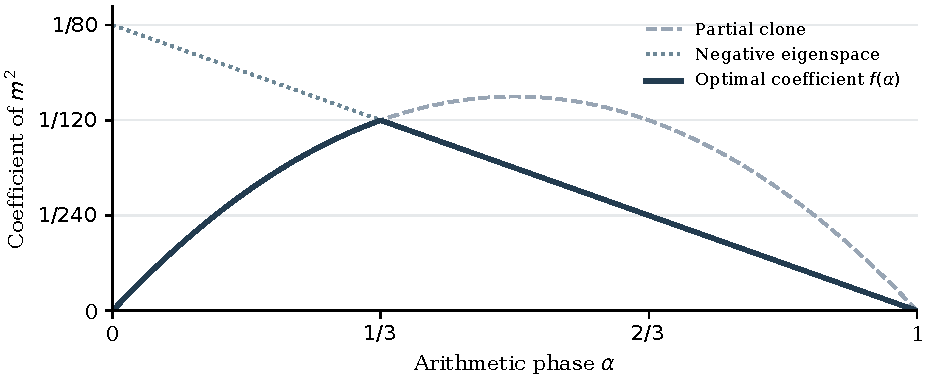
\includegraphics[width=.92\textwidth]{figures/arithmetic_phase.pdf}
 \caption{The second-order coefficient and the two constructions that
 attain it. Their transition is at \(\alpha=1/3\), where
 \(f(\alpha)=1/120\).}
 \label{fig:arithmetic-phase}
\end{figure}

\section{Global extremizers and their variations}

It is useful to allow a finite vertex measure \(\mu\), of total mass
\(s=\mu(\Omega)\), and a symmetric measurable kernel
\(W:\Omega^2\to[0,1]\). All densities in this section are integrated against
\(\mu\). Thus
\begin{align*}
 E&=\frac12\int W(x,y)\,d\mu(x)\,d\mu(y),\\
 C&=\frac1{10}\int
      \prod_{ij\in E(C_5)}W(x_i,x_j)
      \prod_{\substack{i<j\\ij\notin E(C_5)}}(1-W(x_i,x_j))\,d\mu^5.
\end{align*}
Multiplying \(\mu\) by a constant does not change \(C/E^{5/2}\).
Write \(d(x)=\allowbreak\int W(x,y)\,d\mu(y)\) and let \(L(x)\) be the first
derivative of \(C\) with respect to vertex mass at \(x\). Equivalently,
\(L(x)\) is one half of the induced rooted pentagon integral on four
further vertices. A rooted pentagon is always induced throughout the paper.

\subsection{Finite templates and a compact maximization problem}

\begin{lemma}[Finite-template attainment]\label{lem:finite-attainment}
For a fixed finite graph containing an induced pentagon, the supremum of
\(C(H,x)/E(H,x)^{5/2}\) over nonnegative weights with \(E(H,x)>0\) is
attained on a positive-weight induced subgraph.
\end{lemma}
\begin{proof}
Normalize \(E=1\). The square of a pentagon monomial is the product of its
five cyclic edge weights, and is at most \(5^{-5}\) by AM--GM. There are
finitely many such monomials, so the supremum is finite. Take a maximizing
sequence and pass to a subsequence on which every vertex weight converges
in \([0,\infty]\).

If a pentagon contains a weight \(M\to\infty\), its two cyclic neighbors
have weights at most \(1/M\). Its remaining two vertices are adjacent, so
their product is at most one. The pentagon monomial is consequently at
most \(1/M\) and tends to zero. A monomial with only finite limiting
coordinates, one of them zero, also tends to zero. The finite positive
limiting coordinates therefore retain the entire limiting pentagon mass.
Their edge mass is at most one and is positive. If it were strictly less
than one, their ratio would exceed the original supremum. Hence it equals
one, proving attainment.
\end{proof}

\begin{lemma}[A global graphon maximum]\label{lem:global-maximum}
The supremum of \(R\) over all finite graphs, over all finite nonnegative
weighted graphs, and over all positive-density graphons is the same finite
number. It is attained by a graphon of edge density \(1/80\).
\end{lemma}
\begin{proof}
The finite ordinary and weighted suprema agree. Indeed, rational weights
are realized by integer independent blow-ups, and an induced \(C_5\)
cannot use two vertices of one blow-up class: those vertices would be
false twins, whereas \(C_5\) has no false twins. Approximation by rational
weights gives the claim.

At a positive finite-template maximum, remove isolates and normalize the
weights to sum one. Put
\[
 p=2E,\qquad \theta=10C,\qquad
 \kappa=\frac{5C}{2E}=\frac{\theta}{2p}.
\]
The first variation is \(C_i=\kappa d_i\). The elementary universal link
inequality
\begin{equation}
 C_i\le\frac14Ed_i^2\tag{3}
\end{equation}
is proved, including its fractional version, in Lemma~3.1. Since all
active degrees are positive, it implies \(d_i\ge4\theta/p^2\). Averaging
yields
\begin{equation}
 p\ge\frac{16R^2}{1000},\qquad
 R=\sqrt{1000}\,\frac{\theta}{p^{5/2}}.\tag{4}
\end{equation}
In particular the common finite supremum \(M\) is at most
\(\sqrt{1000}/4\), and it is at least \(R_*\) by the Clebsch construction.

Every positive-density graphon has ratio at most \(M\). To see this,
sample independent latent points and then sample edges independently with
the specified probabilities. For any fixed induced pattern, the normalized
injective count converges in probability to its graphon density. The
variance is \(O(1/N)\): pairs of injections on disjoint vertex sets are
independent, and overlapping pairs form an \(O(1/N)\) fraction. Apply this
simultaneously to the edge and induced pentagon counts. The edge density
has a positive limit, so the ratios converge as well.

Conversely, every finite graph with ratio at least \(R_*\) can first be
optimized on its finite template. By (4), the resulting active probability
weighting has edge density at least \(9/500>1/80\). Rescale its active
measure and add isolates to obtain edge density \(1/80\), without changing
its ratio. Thus the supremum over graphons of this fixed density is also
\(M\).

We use the compactness of graphons modulo cut distance
\cite[Theorem~5.1]{LovaszSzegedy2007} and the continuity of fixed
homomorphism densities~\cite{LovaszSzegedy2006}. The induced pentagon
density is continuous as well: expand its five nonedge factors into a
finite alternating sum of ordinary homomorphism densities. The class of
graphons of edge density \(1/80\) is closed and compact, and the
denominator of \(R\) is fixed there. It therefore contains a maximizer.
The sampling argument shows that this is a global maximum over all
positive edge densities, not only over the fixed-density class.
\end{proof}

This globality is essential. Edge variations and insertion of arbitrary
new vertex profiles cannot be inferred merely from optimality of the
weights on a fixed finite template.

\subsection{Vertex and edge variations}

Let \(A(x,y)\) be the induced pentagon completion kernel after one cyclic
edge factor is deleted, and let \(B(x,y)\) be the completion kernel after
one chord nonedge factor is deleted. For explicit conventions, suppressing
the measure symbols,
\begin{align*}
 A(x,y)&=\int W(x,a)W(a,b)W(b,c)W(c,y)\,N_A\,da\,db\,dc,\\
 N_A&=(1-W(x,b))(1-W(x,c))(1-W(y,a))\\
    &\hspace{2em}\cdot(1-W(y,b))(1-W(a,c)),\\
 B(x,y)&=\int W(x,a)W(a,y)W(y,b)W(b,c)W(c,x)\,N_B\,da\,db\,dc,\\
 N_B&=(1-W(x,b))(1-W(a,b))(1-W(a,c))(1-W(y,c)).
\end{align*}
Both kernels are symmetric. Put \(q=A-B\).

\begin{lemma}[Necessary conditions at a global maximum]\label{lem:variations}
At a positive global graphon maximum of \(C/E^{5/2}\), define
\[
 \kappa=\frac{5C}{2E},\quad C''=WA+(1-W)B,\quad
 M=C''-\kappa W,\quad G=\frac{3\kappa}{2E}d\otimes d-M.
\]
Then
\begin{gather}
 L(x)=\kappa d(x)\qquad\text{almost everywhere},\tag{5}\\
 G\succeq0\qquad\text{as an integral operator on \(L^2(\mu)\)},\tag{6}\\
 W(q-\kappa)\ge0,\quad (1-W)(q-\kappa)\le0
       \quad\text{almost everywhere}.\tag{7}
\end{gather}
Consequently
\begin{equation}
 \begin{gathered}
 M\ge B\ge0,\qquad
 \int W(x,y)M(x,y)\,d\mu(y)=\kappa d(x)\\
 \text{almost everywhere}.
 \end{gathered}\tag{8}
\end{equation}
\end{lemma}
\begin{proof}
Replace \(d\mu\) by \((1+sh)\,d\mu\), with \(h\) bounded and \(s\) of
either sign sufficiently small. Normalizing the total measure afterward
does not change the ratio. The first derivative gives (5); the second gives
(6), first for bounded \(h\) and then for all \(h\in L^2(\mu)\) by density.
The kernel of the second vertex derivative is \(WA+(1-W)B\): the two
selected cycle vertices are adjacent in ten ordered positions and
nonadjacent in ten ordered positions, canceling the factor \(1/10\) in
\(C\).

For a bounded symmetric edge perturbation \(H\),
\[
 DC(W)[H]=\frac12\int q(x,y)H(x,y)\,d\mu^2,\qquad
 DE(W)[H]=\frac12\int H(x,y)\,d\mu^2.
\]
Use the feasible one-sided directions \(H=-Wf\) and \(H=(1-W)f\), with
\(f\ge0\). Global maximality yields (7). In particular
\(W(1-W)(q-\kappa)=0\) almost everywhere.

The identity \(M=B+W(q-\kappa)\) proves \(M\ge B\). Furthermore
\[
 \int W(x,y)A(x,y)\,d\mu(y)=2L(x).
\]
Using \(C''=WA+(1-W)B\) and the preceding complementary slackness
identity, we obtain
\begin{align*}
 \int WM
 &=\int WA-\int W(1-W)q-\kappa\int W^2\\
 &=2L-\kappa d=\kappa d.
\end{align*}
This proves (8), including on fractional parts of the graphon.
\end{proof}

On a probability space write
\[
 p=t(K_2,W),\qquad\theta=t_{\mathrm{ind}}(C_5,W).
\]
Multiplying (5) by \(d\), \(d^2\), and
\(b(x)=\int W(x,y)d(y)\,dy\), respectively, gives
\begin{equation}
 p\,t(L_j,W)=\theta\,t(B_j,W),\qquad j=1,2,3.\tag{9}
\end{equation}
Here \(L_1,L_2,L_3\) are an induced pentagon with, respectively, a leaf,
two leaves at the same root, and a pendant path of length two at that root.
Only the five original cycle vertices are required to induce a pentagon;
all other unmentioned pairs are unrestricted. The graphs \(B_1,B_2,B_3\)
are \(P_3,K_{1,3}\), and \(P_4\), with ordinary homomorphism density
conventions.

\subsection{Insertion of a new vertex profile}

For a measurable function \(f:\Omega\to[0,1]\), write \(d(f)=\int f\) and
\begin{equation}
 L(f)=\frac12\int I_{P_4}(a,b,c,d)
                 f(a)f(d)(1-f(b))(1-f(c))\,d\mu^4,\tag{10}
\end{equation}
where
\[
 I_{P_4}=W(a,b)W(b,c)W(c,d)
           (1-W(a,c))(1-W(a,d))(1-W(b,d)).
\]

\begin{lemma}[Profile insertion]\label{lem:profile-insertion}
At a positive global maximum, \(L(f)\le\kappa d(f)\) for every
measurable \(f:\Omega\to[0,1]\).
\end{lemma}
\begin{proof}
Add a new independent class of mass \(\epsilon\), with adjacency profile
\(f\) to the old space. Before normalizing its total measure, the new masses
are
\[
 E_\epsilon=E+\epsilon d(f),\qquad
 C_\epsilon=C+\epsilon L(f)+O(\epsilon^2).
\]
The linear term selects exactly one new cycle vertex. If \(f\) is
fractional, cycles using two new vertices can occur, but their contribution
is still \(O(\epsilon^2)\). Differentiating the ratio in this feasible
direction proves the claim.
\end{proof}

In particular, put \(g=W(u,\cdot)\), \(h=W(v,\cdot)\), and \(f=g(1-h)\).
Combining the lemma with (5) gives
\begin{equation}
 J_\theta(u,v):=L(g)-L(f)
       -\frac{\theta}{2p}\bigl(d(g)-d(f)\bigr)\ge0\tag{11}
\end{equation}
on a probability space. Its removed degree \(d(g)-d(f)=\int gh\) is
nonnegative. Multiplying (11) by the nonnegative factor
\(W(u,v)W(u,z)W(v,z)\) and integrating gives the one profile condition
used in the certificate.

\begin{lemma}[Padding]\label{lem:padding}
Restrict a probability graphon to its positive-degree set and normalize
that restriction to have total measure one. If its edge density is
\(p_a>p_*\), give this normalized active graphon total measure
\(q=\sqrt{p_*/p_a}\) and adjoin isolate mass \(1-q\). The resulting graphon
has the original ratio \(R\) and edge density \(p_*\). If the original
graphon is a global ratio maximum, so is the padded one, and all the
preceding necessary conditions apply.
\end{lemma}
\begin{proof}
Edge mass and pentagon mass scale by the second and fifth powers of the
active measure, respectively. Their normalized ratio is unchanged.
Globality follows from equality of the ratio with the global supremum,
rather than from any restricted variational argument on the original
template.
\end{proof}

\section{A lower bound on the active density}

We work temporarily on a finite measure space \((\Omega,\mu)\) and write
\(S=\mu(\Omega)\). The kernel \(W\) always takes values in \([0,1]\);
rescaling the vertex measure changes neither the ratio \(C/E^{5/2}\) nor
its global maximality. Throughout this section,
\[
 \begin{gathered}
 d(x)=\int_\Omega W(x,y)\,d\mu(y),\qquad
 b(x)=\int_\Omega W(x,y)d(y)\,d\mu(y),\\
 S_2=\int_\Omega d(x)^2\,d\mu(x).
 \end{gathered}
\]
All integrals below are with respect to the indicated powers of \(\mu\).
The vertex derivative of \(C\) is denoted by \(L_x\), and
\(\kappa=5C/(2E)\).

\begin{lemma}[Universal link bounds]\label{lem:universal-links}
For every \([0,1]\)-valued graphon on a finite measure space, set
\begin{align*}
 g_x(u)&=W(x,u),\\
 s_x&=\int_{\Omega^2}g_x(u)(1-g_x(v))W(u,v)\,d\mu(u)\,d\mu(v),\\
 E_{\mathrm{out}}(x)&=\frac12\int_{\Omega^2}
       (1-g_x(u))(1-g_x(v))W(u,v)\,d\mu(u)\,d\mu(v).
\end{align*}
Then
\begin{equation}
 L_x\le\frac{d(x)^2}{4}E_{\mathrm{out}}(x)
       \le\frac{E\,d(x)^2}{4},\tag{12}
\end{equation}
and
\begin{equation}
 L_x\le\frac{s_x^2}{2},\qquad
 E_{\mathrm{out}}(x)=E-\frac{b(x)+s_x}{2}.\tag{13}
\end{equation}
\end{lemma}
\begin{proof}
Fix \(x\) and abbreviate \(g_x\) to \(g\). If
\[
 \Phi(a,b,c,e)=W(a,b)W(b,c)W(c,e)
       (1-W(a,c))(1-W(a,e))(1-W(b,e)),
\]
then the exact rooted link formula is
\[
 L_x=\frac12\int_{\Omega^4}
       \Phi(a,b,c,e)g(a)g(e)(1-g(b))(1-g(c)).
\]
The factor \(1/2\) identifies the two orientations of the rooted pentagon.
For a fixed opposite edge \(bc\), the two endpoint choices have masses
\begin{align*}
 U_{bc}&=\int_\Omega g(a)W(a,b)(1-W(a,c))\,d\mu(a),\\
 V_{bc}&=\int_\Omega g(a)W(a,c)(1-W(a,b))\,d\mu(a).
\end{align*}
The elementary inequality \(u(1-v)+v(1-u)\le1\) for \(u,v\in[0,1]\)
gives \(U_{bc}+V_{bc}\le d(x)\). Dropping the nonedge factor between
the two endpoints and using \(U_{bc}V_{bc}\le d(x)^2/4\) proves the first
inequality in (12). The second follows from \(E_{\mathrm{out}}(x)\le E\).

For the other bound, retain in the link integrand only
\[
 g(a)(1-g(b))W(a,b)\;g(e)(1-g(c))W(e,c).
\]
All discarded factors lie in \([0,1]\). The two remaining pairs integrate
independently, giving \(L_x\le s_x^2/2\). Finally, with
\[
 t_x=\frac12\int_{\Omega^2}g(u)g(v)W(u,v),
\]
we have \(b(x)=2t_x+s_x\) and
\(E_{\mathrm{out}}(x)=E-b(x)+t_x\). These are exactly the last identity
in (13).
\end{proof}

The next estimate uses global maximality. We recall the notation from the
variation formulas: \(A\) and \(B\) are the completions of an induced
pentagon after deleting, respectively, the root edge and the root nonedge.
Put
\[
 M=C''-\kappa W=B+W(A-B-\kappa).
\]
At a global maximizer the first-order, edge, and second-order conditions
give
\begin{equation}
 \begin{gathered}
 L_x=\kappa d(x),\qquad M(x,y)\ge B(x,y)\ge0,\\
 \int_\Omega W(x,y)M(x,y)\,d\mu(y)=\kappa d(x),\\
 G=\frac{3\kappa}{2E}d\otimes d-M\succeq0.
 \end{gathered}\tag{14}
\end{equation}
In particular, after zero-degree points are discarded, Lemma~3.1 implies
\begin{equation}
 d(x)\ge\frac{4\kappa}{E}=\frac{10C}{E^2}
       \quad\text{almost everywhere}.\tag{15}
\end{equation}

\begin{lemma}[A second-order moment inequality]\label{lem:second-order-moment}
At a global maximizer with \(C>0\), on its active finite measure space,
\begin{equation}
 S_2\ge\frac{ES}{3}+\frac{20C}{E}.\tag{16}
\end{equation}
\end{lemma}
\begin{proof}
Write
\[
 \gamma(x,y)=\int_\Omega W(x,z)W(y,z)\,d\mu(z)
\]
for codegree, and let
\[
 Q(x,y)=\int_{\Omega^2}
 W(x,a)W(a,b)W(b,y)(1-W(x,b))(1-W(a,y))\,d\mu(a)\,d\mu(b).
\]
Thus \(Q\) is the completion of an induced three-edge path with its
endpoint nonedge factor omitted. In \(B(x,y)\), delete the two nonedge
factors joining the common neighbor to the internal vertices of this path.
This gives
\[
 B(x,y)\le\gamma(x,y)Q(x,y).
\]
Define
\[
 D=\int_{\Omega^2}(1-W)Q=t_{\mathrm{ind}}(P_4,W),\qquad
 L_0=\int_{\Omega^2}(1-W)B\gamma.
\]
Since \(\int(1-W)B=10C\), Cauchy--Schwarz yields
\begin{equation}
 100C^2\le DL_0.\tag{17}
\end{equation}
Here \(B/\gamma\) may be assigned the value zero where \(\gamma=0\);
the bound \(B\le\gamma Q\) makes this convention harmless.

We also have
\begin{equation}
 D\le E^2.\tag{18}
\end{equation}
Indeed, fix the two outer edges on four independent points. Of the four
possible cross edges, the probabilities that exactly one is present sum
to at most one. Each choice, after integration, is the same induced-\(P_4\)
density \(D\). Consequently \(4D\le(\int W)^2=4E^2\). This proof applies
directly to fractional values of \(W\).

Let \(T\) be the integral operator with kernel \(W\). We now justify an
optimized diagonal test of the positive operator \(G\) in (14). Fix a
bounded real function \(z\), and choose increasing finite measurable
partitions whose conditional expectations of \(W,M,d,z\) converge in
\(L^2\), using the product partitions for the two kernels. Such partitions
exist by approximating the kernels by finite linear combinations of
measurable rectangles and the functions by simple functions, then
successively refining all the sets that occur. Let \(P_n\) denote
orthogonal projection onto the associated step functions, and set
\[
 T_n=P_nTP_n,\qquad M_n=P_nMP_n,\qquad d_n=P_nd.
\]
These are compressions of the original kernels, not derivatives recomputed
at an approximating graphon. In particular
\[
 G_n=\frac{3\kappa}{2E}d_n\otimes d_n-M_n\succeq0.
\]
Put \(z_n=P_nz\) and let \(Z_n\) be
multiplication by \(z_n\) on the finite-dimensional step space. The matrix
\((T_n-Z_n)^2\) is positive semidefinite, so
\[
 \operatorname{tr}\bigl(M_n(T_n-Z_n)^2\bigr)
       \le\frac{3\kappa}{2E}\|(T_n-Z_n)d_n\|_2^2.
\]
In the orthonormal basis \(\mathbf1_U/\sqrt{\mu(U)}\) of partition cells,
each diagonal entry of \(M_n\) is nonnegative because \(M\ge0\).
Therefore \(\operatorname{tr}(M_nZ_n^2)\ge0\), and discarding this term
gives
\begin{equation}
 \operatorname{tr}(M_nT_n^2)
 \le\frac{3\kappa}{2E}\|T_nd_n-Z_nd_n\|_2^2
                 +2\operatorname{tr}(M_nT_nZ_n).\tag{19}
\end{equation}
We explain all three limits. Conditional expectations of the bounded
kernels converge in Hilbert--Schmidt norm, so
\(\operatorname{tr}(M_nT_n^2)\to\operatorname{tr}(MT^2)\). Also
\(T_nd_n-Z_nd_n\to b-zd\) in \(L^2\): the kernels, \(d_n\), and \(z_n\)
are uniformly bounded, and the conditional expectations converge in
\(L^2\). Finally, if the same symbols denote the step kernels, the mixed
trace is
\[
 \operatorname{tr}(M_nT_nZ_n)
   =\int_{\Omega^2}z_n(x)M_n(x,y)W_n(x,y)\,d\mu(x)\,d\mu(y).
\]
The integrands converge in \(L^1\), and (14) identifies the limit as
\(\kappa\int zd\). No infinite-dimensional trace involving the arbitrary
multiplication operator \(Z^2\) is required; its nonnegative contribution
was discarded before taking a limit.

The kernel of \(T^2\) is \(\gamma\ge0\). Since \(M\ge B\),
\[
 \operatorname{tr}(MT^2)=\int_{\Omega^2}M\gamma
       \ge\int_{\Omega^2}(1-W)B\gamma=L_0.
\]
Passing to the limit in (19) gives
\begin{equation}
 L_0\le\kappa\int_\Omega
       \left[\frac{3}{2E}(b-zd)^2+2zd\right]\,d\mu.\tag{20}
\end{equation}
Choose
\[
 z(x)=\frac{b(x)-2E/3}{d(x)}.
\]
This is bounded: \(b/d\le S\), and the positive lower bound (15)
controls \(1/d\) on the active space. The choice minimizes the scalar
quadratic in (20), yielding
\[
 L_0\le\kappa\left(2\int_\Omega b\,d\mu-\frac{2ES}{3}\right)
       =2\kappa\left(S_2-\frac{ES}{3}\right).
\]
Combine this with (17) and (18), and use \(\kappa=5C/(2E)\).
The result is (16).
\end{proof}

\begin{proposition}[Active density]\label{prop:active-density}
Let \(W\) be a global maximizer of \(C/E^{5/2}\) among graphons of
positive edge density. Suppose
\[
 5^{5/2}\frac{C}{E^{5/2}}\ge\frac{3}{2\sqrt2}.
\]
After its zero-degree set is deleted and the remaining measure is
normalized to one, its edge density satisfies
\begin{equation}
 p_{\mathrm{act}}\ge
 \frac{80000}{(491\sqrt{10}-75\sqrt2)^2}>\frac5{144}.\tag{21}
\end{equation}
\end{proposition}
\begin{proof}
Delete zero-degree points, which changes neither \(E\) nor \(C\), and
rescale the measure so that \(E=1\). Write \(c=C\) in this normalization,
so \(c\ge c_*=3/(50\sqrt{10})\) and \(\kappa=5c/2\). By (15),
\begin{equation}
 d(x)\ge\delta:=10c,\qquad S\le\frac1{5c}.\tag{22}
\end{equation}
The second inequality uses \(\int d=2\).

Put
\[
 T_0=\int_\Omega d(x)b(x)\,d\mu(x),\qquad
 V=\int_\Omega d(x)s_x\,d\mu(x).
\]
The inequality
\(d(x)d(y)\ge\delta(d(x)+d(y))-\delta^2\), integrated against \(W(x,y)\),
and Lemma~3.2 give
\begin{equation}
 T_0\ge2\delta S_2-2\delta^2
       \ge\frac{20}{3}cS+200c^2.\tag{23}
\end{equation}
Here \(\delta\) is the fixed bound \(10c\), so no substitution is made in
a nonmonotone function of the actual minimum degree. By
\(L_x=\kappa d(x)\) and (13), \(s_x\ge\sqrt{2\kappa d(x)}\).
Jensen's inequality therefore gives
\begin{equation}
 V\ge\sqrt{2\kappa}\int_\Omega d(x)^{3/2}\,d\mu(x)
       \ge4\sqrt{\frac{\kappa}{S}}.\tag{24}
\end{equation}
Divide the first inequality in (12) by \(d(x)>0\), use
\(L_x=\kappa d(x)\), and integrate. With
\(E_{\mathrm{out}}(x)=1-(b(x)+s_x)/2\) this reads
\[
 8\kappa S+T_0+V\le4.
\]
Equations (23) and (24) now imply
\[
 \frac{40}{3}cS+100c^2+2\sqrt{\frac{\kappa}{S}}\le2.
\]
The mass bound in (22) gives \(2\sqrt{\kappa/S}\ge5\sqrt2\,c\), and hence
\[
 S\le\frac3{20c}-\frac{15}{2}c-\frac{3\sqrt2}{8}.
\]
The right-hand side is strictly decreasing for \(c>0\). Substituting
\(c_*=3/(50\sqrt{10})\) yields
\[
 S\le\frac{491\sqrt{10}-75\sqrt2}{200}.
\]
Since \(11\sqrt{10}<75\sqrt2\), this upper bound is strictly less than
\(480\sqrt{10}/200=\sqrt{288/5}\). On normalizing the active measure to
one, its edge density is \(p_{\mathrm{act}}=2/S^2\). This proves both
inequalities in (21).
\end{proof}

In particular, a global maximizer can be padded by isolated mass to the
rational density \(p_*=5/144\). The same conclusion applies to any
equality graphon once the sharp bound has been established: such a graphon
is itself a global maximizer. Thus the padding needed for the equality
analysis does not require a finite-support or a \(\{0,1\}\)-valued
assumption.

\section{A single exact certificate}

We work on a probability space and write
\[
 p=t(K_2,W),\qquad\theta=t_{\mathrm{ind}}(C_5,W),\qquad
 p_*=\frac5{144},\qquad\tau=\frac5{663552}.
\]
Balanced Clebsch on an active set of measure \(1/3\), with isolates outside
it, has \((p,\theta)=(p_*,\tau)\). The certificate in this section applies
to arbitrary graphons of density \(p_*\); its variational interpretation
is used at a global maximum.

\subsection{The additional variational columns}

Retain the partially induced patterns \(L_j\) and the graphs \(B_j\) from
(9), and abbreviate
\[
 \Phi_j(s)=p_*t(L_j,W)-s\,t(B_j,W),\qquad j=1,2,3.
\]
We retain four additional columns. We describe them explicitly to specify
their signs and their dependence on the target density. Two have zero
multipliers in the supplied certificate.

First let \(z(x)=2L(x)\) be the rooted labeled induced-pentagon density,
and put
\[
 T(x)=\int W(x,y)W(x,w)W(y,w)\,dy\,dw,
\]
\[
 L_\triangle=\int z(x)T(x)\,dx,\qquad
 B_\triangle=\int d(x)T(x)\,dx.
\]
Equivalently, \(L_\triangle\) is the partially induced pattern obtained
by attaching a triangle at one vertex of an induced pentagon, and
\(B_\triangle\) is the ordinary density of a triangle with a leaf at its
root. Define
\[
 \Phi_\triangle(s)=p_*L_\triangle-sB_\triangle.
\]
Multiplying the first-order identity by \(T(x)\) gives
\(\Phi_\triangle(\theta)=0\), and \(B_\triangle\ge0\).

For the next two columns, fix ordered roots \(u,v\), write \(g=W(u,\cdot)\)
and \(h=W(v,\cdot)\), and set
\begin{align*}
 \psi_0(u,v)&=\int g(x)h(x)g(y)h(y)(1-W(x,y))\,dx\,dy,\\
 \psi_1(u,v)&=\int g(x)h(x)g(y)h(y)W(x,y)\,dx\,dy.
\end{align*}
Conditional on the root edge being present, these are the probabilities of
a diamond with its two degree-three vertices rooted, and of a complete
four-vertex graph. Using the completion kernels \(A,B\) from Section~2,
define
\[
 J_i(s)=\int W(u,v)\psi_i(u,v)
       \left(A(u,v)-B(u,v)-\frac{s}{2p_*}\right)\,du\,dv,
       \qquad i=0,1,
\]
and \(R_i=\int W(u,v)\psi_i(u,v)\,du\,dv\ge0\).
The existing-edge condition (7) gives \(J_i(\theta)\ge0\) at a global
maximum.

Finally, let \(J_{\mathrm{del}}(s)\) be the integral of the expression
in (11), with \(\theta\) replaced by \(s\), against
\(W(u,v)W(u,w)W(v,w)\,du\,dv\,dw\).
Thus \(J_{\mathrm{del}}(\theta)\ge0\). Its removed-degree coefficient is
\[
 D_{\mathrm{del}}=\int W(u,v)c(u,v)^2\,du\,dv\ge0,\qquad
 c(u,v)=\int W(u,x)W(v,x)\,dx.
\]
In particular \(D_{\mathrm{del}}=R_0+R_1\). At fixed edge density,
\begin{equation}
 \begin{aligned}
 \Phi_j(\tau)&=(\theta-\tau)t(B_j,W),
 &\Phi_\triangle(\tau)&=(\theta-\tau)B_\triangle,\\
 J_i(\tau)&=J_i(\theta)+\frac{\theta-\tau}{2p_*}R_i,
 &J_{\mathrm{del}}(\tau)&=J_{\mathrm{del}}(\theta)
                  +\frac{\theta-\tau}{2p_*}D_{\mathrm{del}}.
 \end{aligned}\tag{25}
\end{equation}
The first line uses the vertex first-order conditions. All added
coefficients of \(\theta-\tau\) in the second line are nonnegative.

\subsection{Seven-vertex coefficients and flag squares}

There are \(1044\) unlabeled simple graphs on seven vertices. Their
canonical adjacency masks, edge lists and orbit sizes are supplied with
the certificate. Write \(\pi_H(W)\) for the probability that seven
independent graphon samples induce \(H\). For a pattern on \(r\le7\)
labeled vertices, specify its required edges and nonedges; all other
pairs are unrestricted. Its coefficient on \(H\) is the number of
injections satisfying these requirements divided by \((7)_r\).
Averaging this coefficient against \(\pi_H(W)\) gives its graphon density
exactly. In particular the induced-pentagon coefficient is \(I_5(H)/252\).

The five rooted flag spaces are as follows.
\begin{center}
\begin{tabular}{lrrrr}
\toprule
Root type & Roots & Flag order & Flags & Denominator\\
\midrule
One root & 1 & 4 & 20 & 140\\
Three independent roots & 3 & 5 & 72 & 1260\\
Edge and isolated root & 3 & 5 & 72 & 1260\\
Path \(01,12\) & 3 & 5 & 72 & 1260\\
Triangle & 3 & 5 & 72 & 1260\\
\bottomrule
\end{tabular}
\end{center}
Root labels are fixed individually. Isomorphisms may permute only the
extension vertices. For each host, sample an ordered root embedding and
two disjoint extension sets. Cross-edges between the two extensions are
unrestricted. The sampling denominators are
\(7\binom63=140\) and \((7)_3\binom42=1260\).

For a flag vector \(v\), let \(q_F(x)\) be its conditional flag
probabilities at a root tuple and let \(P_\sigma(x)\) be the probability
of the root type. The associated square is
\begin{equation}
 Q_v(W)=\int P_\sigma(x)\left(\sum_Fv_Fq_F(x)\right)^2\,dx\ge0.\tag{26}
\end{equation}
The root-type factor occurs once. This convention is essential for
fractional graphons. An individual finite host matrix need not be positive
semidefinite; its average over \(\pi_H(W)\) is the matrix represented by
(26).

For clarity, the raw source counts use the injection denominator \((7)_r\)
for a pattern on \(r\) labeled vertices. Thus the cycle and house
completions in \(J_i\), and \(L_\triangle\), use \(5040\);
\(R_i\), \(B_\triangle\), and \(D_{\mathrm{del}}\) use \(840\).
The link difference in \(J_{\mathrm{del}}\) uses
\(10080=2\cdot7!\), including the \(1/2\) in the rooted link (10).
Internal symmetries permit cancellations in some of these fractions, but
the data files retain the raw injection counts. Each expanded profile term
is multilinear in the formal graph-edge variables, so Boolean-host
averaging is valid also for fractional \(W\).

\begin{proposition}[Exact finite identity]\label{prop:finite-certificate}
For every graphon of density \(p_*\) there is the identity
\begin{equation}
 \begin{aligned}
 &\tau-\theta-\sum_{j=1}^3\lambda_j\Phi_j(\tau)
       -\lambda_\triangle\Phi_\triangle(\tau)
       -\sum_{i=0}^1a_iJ_i(\tau)-a_{\mathrm{del}}J_{\mathrm{del}}(\tau)\\
 &\hspace{3em}
       =\sum_{r=1}^{184}b_rQ_{v_r}(W)+\sum_Hs_H\pi_H(W).
 \end{aligned}\tag{27}
\end{equation}
Here \(\lambda_\triangle,a_{\mathrm{del}},b_r\) are strictly positive
rational numbers, \(a_0=a_1=0\), and \(s_H\ge0\). Exactly \(826\) host
slacks are positive. The three unrestricted first-order multipliers
satisfy the exact inequalities
\begin{equation}
 -\frac{1157}{10}<\lambda_1<0,\qquad
 \lambda_3<0,\qquad\lambda_2+\lambda_3>310.\tag{28}
\end{equation}
All rational coefficients and integer flag vectors are specified in
\texttt{\upshape all\_\allowbreak graph\_\allowbreak exact\_\allowbreak certificate.json}.
\end{proposition}
\begin{proof}
The supplied identity has one row for each of the \(1044\) hosts.
Besides the displayed columns, its finite form includes the \(34\)
unrestricted fixed-density identities
\(p_F(W)t(K_2,W)-p_*p_F(W)\), one for each unlabeled graph \(F\) on
five vertices, where \(p_F\) is its induced-graph probability.
Their sum is \(t(K_2,W)-p_*\), so this basis is equivalent to that
single identity together with any \(33\) of the five-vertex identities.
In the finite coefficients the additional edge is sampled disjointly
from the vertices of \(F\). These columns vanish after graphon averaging
at density \(p_*\).

The checker computes the entire host atlas, all five flag matrices,
the partially induced patterns and all the additional columns from their
edge requirements. It then computes every declared source column and
verifies the \(1044\) rational identities and every required coefficient
sign exactly. Clearing one
common denominator reduces the final identity check to integer arithmetic.
The rational comparisons in (28) are checked in the same way. Thus
averaging the finite identities proves (27); the numerical search used
to find the coefficients is not part of the verification.
\end{proof}

\subsection{A uniformly positive slope}

Put \(x=t(P_3,W)\), \(y=t(K_{1,3},W)\) and \(z=t(P_4,W)\).
For every graphon,
\[
 z=\int W(u,v)d(u)d(v)\,du\,dv
 \le\frac12\int W(u,v)\bigl(d(u)^2+d(v)^2\bigr)\,du\,dv=y,
\]
and Cauchy--Schwarz gives \(x^2\le py\). Consequently
\begin{equation}
 \begin{aligned}
 1+\lambda_1x+\lambda_2y+\lambda_3z
 &\ge1+\lambda_1x+(\lambda_2+\lambda_3)y\\
 &\ge1+\lambda_1x+\frac{\lambda_2+\lambda_3}{p_*}x^2\\
 &\ge1-\frac{p_*\lambda_1^2}{4(\lambda_2+\lambda_3)}
 >\frac{2232551}{3571200}>\frac58.
 \end{aligned}\tag{29}
\end{equation}
The penultimate comparison uses (28).

\begin{corollary}[Bound at a global maximum]\label{cor:certificate-bound}
A positive global maximum of the induced-pentagon to edge ratio,
normalized to edge density \(p_*\), satisfies \(\theta\le\tau\).
If \(\theta=\tau\), all \(184\) ordinary squares in (27) vanish.
\end{corollary}
\begin{proof}
Insert (25) into (27). The resulting identity is
\[
 \begin{aligned}
 (\tau-\theta)\mathcal B(W)
 &=\sum_rb_rQ_{v_r}(W)+\sum_Hs_H\pi_H(W)\\
 &\quad+\sum_{i=0}^1a_iJ_i(\theta)
              +a_{\mathrm{del}}J_{\mathrm{del}}(\theta),
 \end{aligned}
\]
where
\[
 \mathcal B(W)=1+\sum_j\lambda_jt(B_j,W)
       +\lambda_\triangle B_\triangle
       +\frac{a_0R_0+a_1R_1+a_{\mathrm{del}}D_{\mathrm{del}}}{2p_*}.
\]
The last two contributions to \(\mathcal B\) are nonnegative, so (29)
gives \(\mathcal B>5/8\). Every term on the right is nonnegative at a
global maximum. This proves the bound and, at equality, the vanishing
of each ordinary square, since all \(b_r\) are strictly positive.
\end{proof}

\subsection{Exact spans for equality}

We record three finite consequences of this same certificate. Each is an
explicit rational linear combination, checked coordinate by coordinate;
no numerical rank assertion is used.

\begin{lemma}[Triangle domination]\label{lem:triangle-domination}
In the path type with root edges \(01,12\) and extension vertices \(3,4\),
there is a vector \(G\) in the rational span of its \(53\) strictly
positive square vectors such that
\[
 G(F)=0\quad\text{if \(F\) is triangle-free},\qquad
 G(F)\ge1\quad\text{if \(F\) contains a triangle}.
\]
There are \(24\) coordinates of the first kind and \(48\) of the second.
\end{lemma}
\begin{proof}
The combination is specified in the supplied file
\begin{center}
 \texttt{all\_graph\_path3\_triangle\_domination\_span.json}.
\end{center}
Its checker computes which of the \(72\) flags contain a triangle,
checks that every source vector comes from a strictly positive square
of the final certificate, and adds the rational combination in every
coordinate. The result is zero on all \(24\) triangle-free coordinates
and at least one on all other coordinates. In the supplied witness,
\(G\) is itself a positively weighted source vector: it is the indicator
of the \(48\) triangle-containing flags.
\end{proof}

Once triangle-freeness has been established, only triangle-free flag
coordinates contribute to a conditional flag distribution. The following
two span identities concern the restrictions of the same all-graph square
vectors to those coordinates.

\begin{lemma}[Degree span]\label{lem:degree-span}
In the triangle-free flags of the path type \(01,12\), the vector
\begin{equation}
 g(F)=24\bigl(e_F(1,3)+e_F(1,4)\bigr)-5\tag{30}
\end{equation}
lies in the rational span of the restricted strictly positive square
vectors of that type.
\end{lemma}
\begin{proof}
The witness in
\texttt{all\_graph\_tf\_degree\_codegree\_spans.json} uses \(22\) nonzero
coefficients from the \(53\) path-type sources. The independent checker
identifies the \(24\) triangle-free flags from their edge sets and verifies
(30) in all \(24\) coordinates by rational addition. All source squares
have strictly positive rational weights.
\end{proof}

\begin{lemma}[Codegree span]\label{lem:codegree-span}
Consider the triangle-free flags of the type with the single root edge
\(01\) and isolated root \(2\). Put
\[
 h_i(F)=24\bigl(e_F(i,3)+e_F(i,4)\bigr)-5,\qquad i=0,1.
\]
For each \(i=0,1\), the vector
\begin{equation}
 k_i(F)=5\sum_{j=3}^4e_F(i,j)e_F(2,j)
                 -2\sum_{j=3}^4e_F(2,j)\tag{31}
\end{equation}
lies in the rational span of \(h_0,h_1\) and the restricted strictly
positive square vectors of this type.
\end{lemma}
\begin{proof}
The same witness file gives two explicit combinations, each with \(30\)
nonzero coefficients. Their available sources are the \(56\) positive
edge-type square vectors and the two degree rows \(h_0,h_1\). The checker
computes those rows and the targets (31) from the flag edge sets,
then verifies both identities in all \(32\) triangle-free coordinates.
These are consequences of the single \(1044\)-host certificate; no
separate triangle-free extremal certificate is required.
\end{proof}

\section{The sharp inequality}

\begin{proof}[Proof of the inequalities in Theorems 1.1 and 1.3]
Let \(M\) be the common supremum supplied by Lemma~2.2, and choose a
global graphon maximum attaining it. The Clebsch construction gives
\(M\ge R_*\). Proposition~3.3 shows that its active probability edge
density is strictly greater than \(p_*=5/144\). Lemma~2.5 therefore
produces a global maximum at edge density \(p_*\). All vertex, edge, and
profile conditions used in the exact certificate hold at this graphon.

At fixed density \(p_*\), a ratio at least \(R_*\) is equivalent to
\(\theta\ge\tau\). Corollary~4.2 gives \(\theta\le\tau\), so \(M=R_*\).
By the definition of \(M\), the bound holds for every positive-density
graphon and for every finite nonnegative weighted graph. If the edge mass
is zero, the induced pentagon mass is zero as well. The Clebsch
construction verifies sharpness.
\end{proof}
